\chapter{Introduction}

	\section{What is PCG?}
Level design is a crucial factor in video games that has been around for as long as games have. It consists of manually designing an environment by specifically defining every bit of detail and importing them directly into the game. Such details include, but are not limited to: Terrain shape, goals or mission objectives, location of enemies and collectible objects. This is called {\em level designing}, and it's traditionally done by a human-being known as an {\em artist} or {\em game designer}.

However, level designing is not the only method to create the virtual environment of a video game. Another method is to procedurally generate a virtual environment. The concept behind this method is to write an algorithm that will design a level by using randomly generated numbers as opposed to leaving the task to a human. This is called {\em level generation}. This can greatly increase the amount of content or the value of a game. For this reason, it is not uncommon for games to include this method. Naturally, this procedural method differs greatly from traditional level designing that is more directed towards an artistic path.

Procedural Content Generation (PCG) is the general term used to describe the creation of any random computer-designed objects within a game. PCG can refer to the creation of any kind of randomised object, such as non-playable characters (NPCs), the weapons they can use, and so forth. Although generally speaking, PCG refers to the generation of the game's environment, such as creating a randomised mountain terrain or maze for example.

In the course of this dissertation, the focus will be targeted towards the creation of the environment itself, more specifically, to creation of a maze or a dungeon.

	\section{A short history}
Level generation is not particularly a new concept. It has been around for a significant amount of time and has been implemented in a number of games.

	\subsection{Rogue-like games}

With regards to dungeon-generation, the most popular example is probably {\em Rogue}, a game created in the 1980s \citep{DBLP:journals/tciaig/AshlockLM11}. This game was the first of its kind and was evidently a big success. Later on, many games like {\em Diablo}, {\em NetHack}, {\em Moria} and {\em Dwarf Fortress} \citep{DBLP:conf/cig/TogeliusPBWHY10} followed the same style but improved the features of Rogue. These types of games are generally referred to as {\em rogue-like} games.
\begin{figure}[h!]
\centering
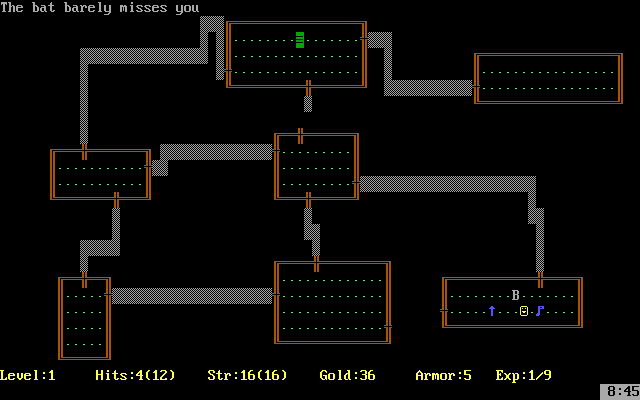
\includegraphics[width=0.50\textwidth]{images/Rogue0.png}
\caption{A screenshot of the console-based game {\em Rogue}.
\\{\footnotesize http://tripalot.com/roguelike/img/rogue.gif} }
\end{figure}

NetHack had improved on Rogue by adding more detail to the dungeons. The game itself would take up about 2 MB of disk space, which at that time was considered a lot. Due to the level of detail in NetHack, it was found to be far less predictable and more enjoyable than Rogue. The amount of content in NetHack is probably what made it so successful \citep{Roguelike}.
\begin{figure}[h!]
\centering
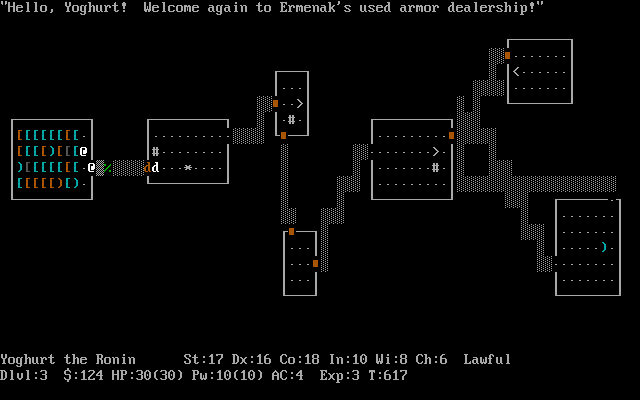
\includegraphics[width=0.50\textwidth]{images/nethack.png}
\caption{{\em HetHack}, a successor of Rogue.
\\{\footnotesize http://tripalot.com/roguelike/img/nethack.gif} }
\end{figure}

Moria also improved upon Rogue by adding an exceedingly large amount of content, even more than NetHack. It had more monsters, more spells, more items and etc., taking this genre of games to the next level \citep{Roguelike}.
\begin{figure}[h!]
\centering
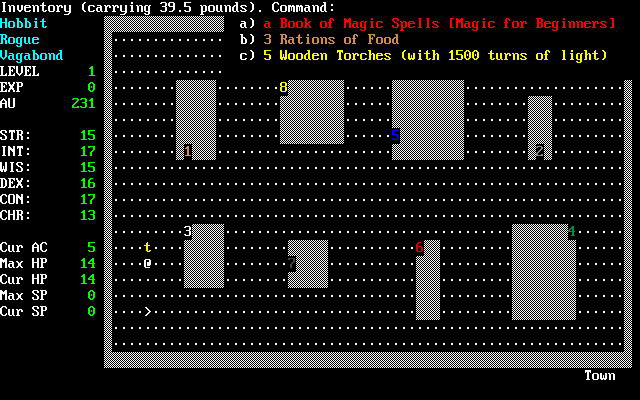
\includegraphics[width=0.50\textwidth]{images/moria.png}
\caption{A screenshot of {\em Moria} (a.k.a. {\em Angband}).
\\{\footnotesize http://tripalot.com/roguelike/img/angband.gif} }
\end{figure}

	\subsection{Other games}
Some games such as Borderlands and Left 4 Dead have pseudo-random levels, meaning that the overall layout of the game's level is designed by hand but contains some randomised features \citep{DBLP:journals/tciaig/TogeliusYSB11}. Other games such as Diablo completely discarded level designing and randomly generated all the levels, NPCs and props \citep{Nitsche-CaseStudy}.

One notable example is Minecraft, a game originally designed by the Swedish developer Markus Persson (a.k.a ``Notch") who later founded the game studio Mojang \footnote{http://www.minecraft.net/game/credits (Date accessed: 28th Feburary)}. In Minecraft, the player is placed in a world composed of different types of blocks. The blocks are placed at random using Perlin noise \footnote{http://pcg.wikidot.com/pcg-games:minecraft (Date accessed: 28th Feburary)}. The wide range of block types allows the player to experience different biomes.  The world is pseudo-infinite; meaning that, as the player moves into unexplored areas, the game will automatically generate more content to fill that area.
\begin{figure}[h!]
\centering
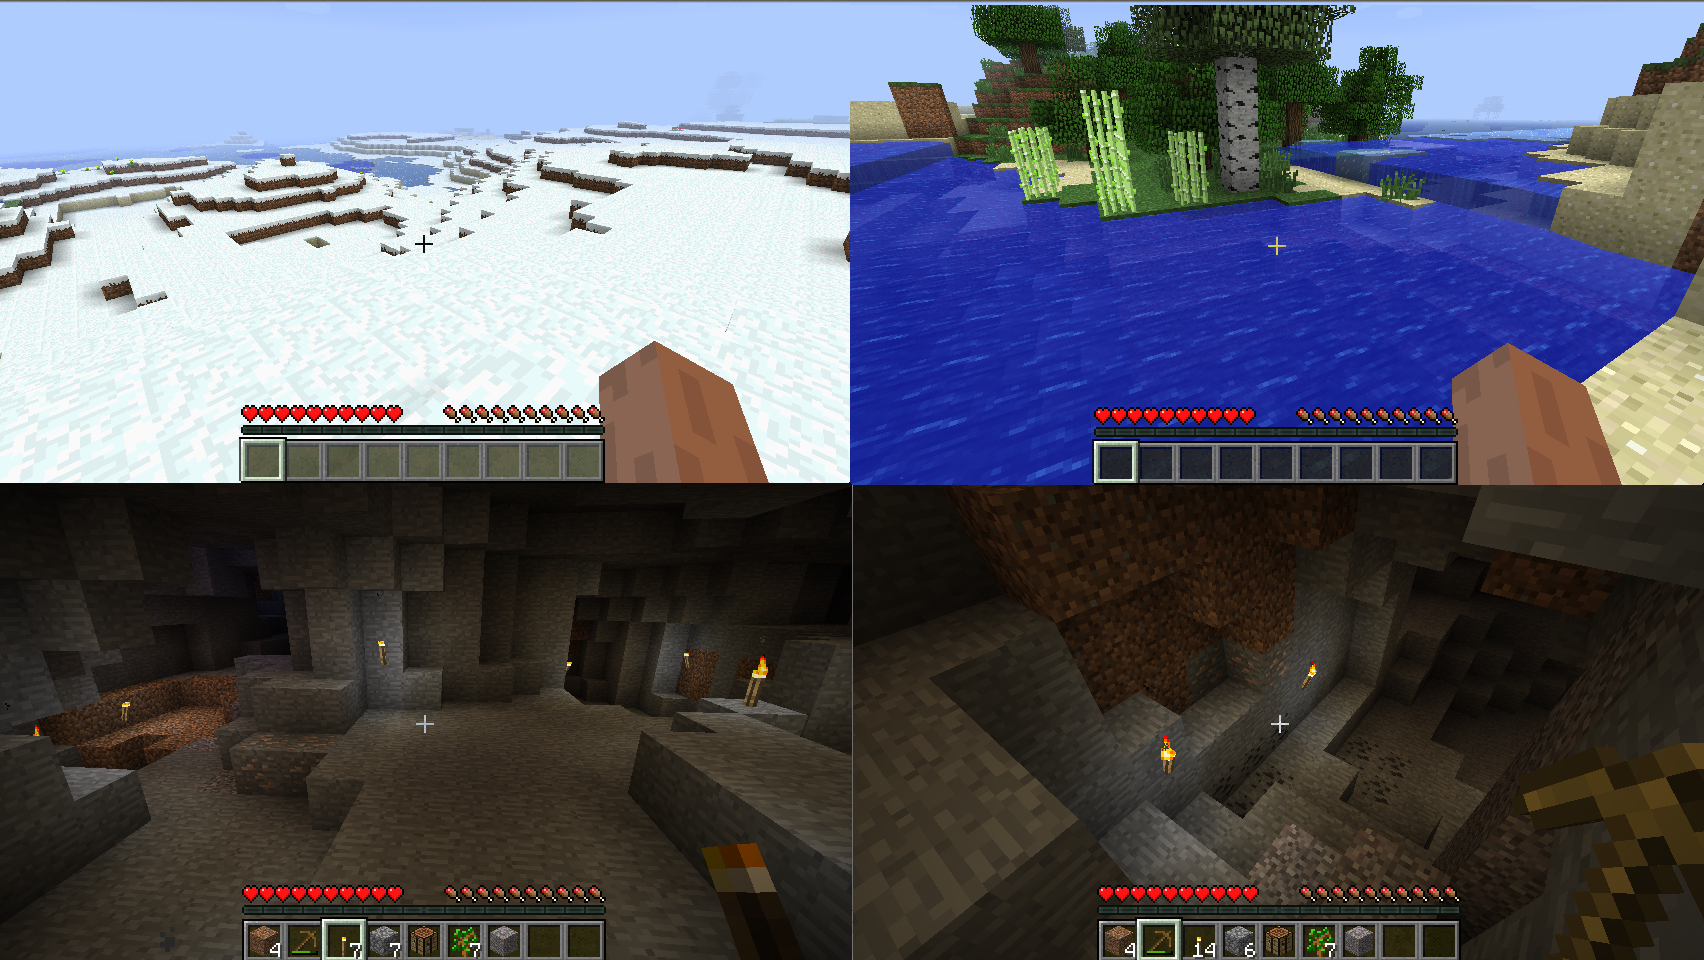
\includegraphics[width=0.92\textwidth]{images/minecraft.png}
\caption{Procedural level design in Minecraft.}
\end{figure}

A game similar to Minecraft that also uses PCG is Terraria. Like Minecraft, it also revolves around randomly positioned blocks, with the main difference being that it's a 2D game. Terraria is a lot more focused on generating content other than terrain. In Terraria players can encounter numerous different types of enemies. They can also find treasures in vases and chests that are randomly scattered across the world.
\begin{figure}[h!]
\centering
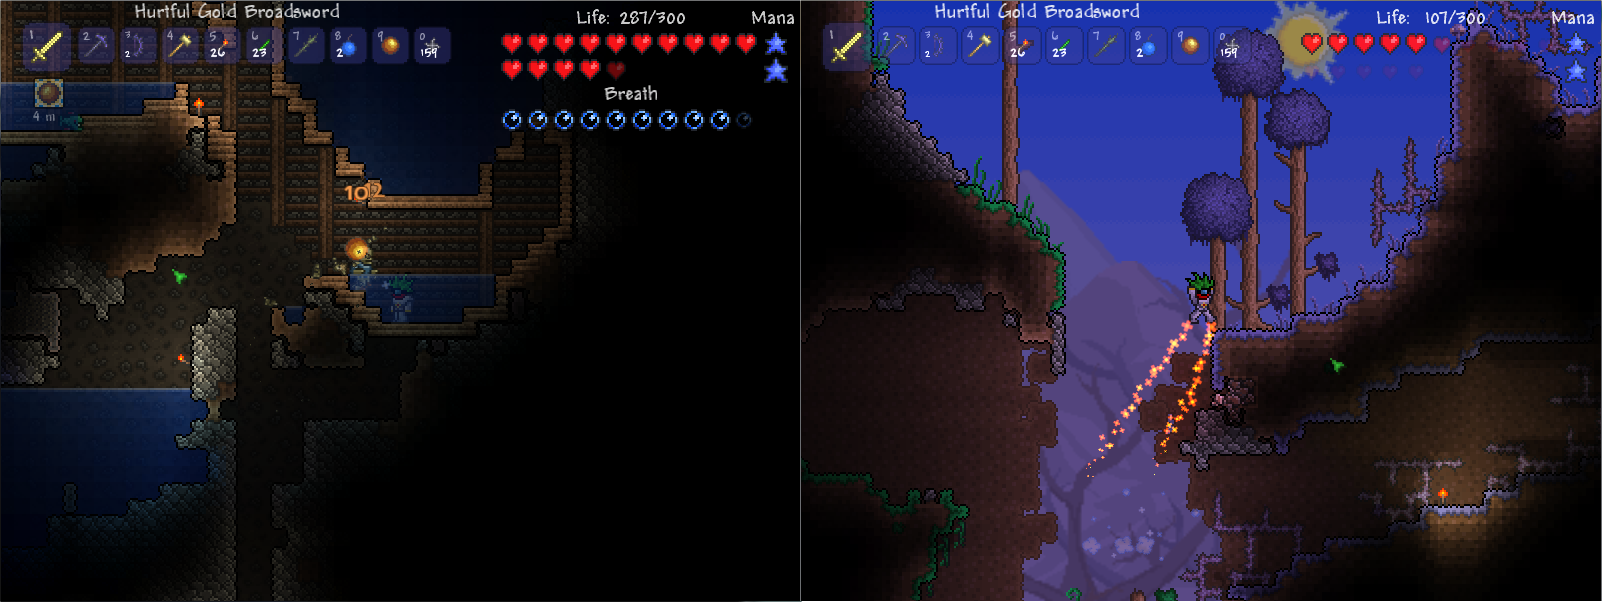
\includegraphics[width=0.6\textwidth]{images/terraria.png}
\caption{Terraria is a 2D game inspired by Minecraft which also utilises PCG.}
\end{figure}

	\section{Advantages}
The programmatic approach presents various advantages over level designing. The two major advantages are:
\begin{enumerate}
\item {\bf Time:} Naturally, level designing is a very time-consuming process. However, computers are much faster than humans. Once a good level generator is developed, it can potentially generate an infinite amount of levels in a very short time-span. 

\item {\bf Amount of content:} As a direct result from the time constraint, level generation offers far more content. Video games with a fixed level design offer far less re-playability than those with procedural level generation because the game will get boring and predictable after a while. Level generation can allow a completely different feel to the game every-time it's played and can offer seemingly endless content \citep{DBLP:conf/aiide/ComptonM06}.
\end{enumerate}

Notably, other minor advantages can emerge from this programming approach. For instance, the total memory consumption of the game when distributed could be less, because content is generated on the fly when needed and doesn't have to be packed in the distribution medium \citep{DBLP:journals/tciaig/TogeliusYSB11}.


	\section{Disadvantages}
Although PCG can makes things interesting in a video game there are major downsides to it:
\begin{enumerate}
\item {\bf Unrealic:} Because the levels are generated at random by a computer they are effectively only mimicking a real-life environment. Real-life scenarios are too complex to express and are therefore based on approximate models. If these models are not accurate enough then generated content will have obvious unrealistic features.

\item {\bf Specificity:} The behaviour of a content generation algorithm should be specific to the desired result. For example: generating a natural environment such as a forest will require an algorithm that is substantially different to an algorithm used to generate a city. Generalisation is not always possible and environments with mixed characteristics will have to incorporate multiple techniques, making them more complex.

\item {\bf Repetition:} PCG algorithm generally rely on pre-defined assets of sorts to increase the realism of an environment. For example: an algorithm used to generate a desert would probably utilise some artwork, such as one or more sand pictures to diffuse a texture. Even if the algorithm doesn't use any artwork then the formulas used to model the environment will generate sections that are noticeably similar.
\end{enumerate}

All of these issues can be reduced in some ways. To make the environment more realistic, we need to rely on a lot of artwork to make the result more convincing. However, if we rely too much on pre-determined assets then it will increase repetition and the generated content will lose its uniqueness. We cannot produce an infinite amount of pre-determined assets and must rely on mathematical functions with a wide range to effectively reduce repetition. As for specificity, the best way to counter this is to write base code that can be extended by different algorithms.


	\section{Statement of Problem and Aims}
We know now that PCG can potentially be advantageous to game developers. PCG suffers from three major issues and amongst those there is one that seems to be more neglected than others: Specificity. Maximising realism whilst reducing repetition tends to be the priority for game developers because those two issues directly affect the visual quality of game. 

In this thesis, the primary focus will be to keep the algorithm as general as possible. In order words, the problem of specificity will be tackled more directly than the others. The aim of the project is to conceive a framework that is entirely independent and capable of being re-used in any game that requires that kind of environment. The framework should be able to support the following key features:
\begin{itemize}
\item Using a solid mathematically to model generate dungeon-like environments. This model should be abstract and extendible.
\item Procedurally model the generated environment into a 3D mesh.
\item Render the environment and provide means for the user to interact with the environment.
\end{itemize}